
\chapter{cuBLAS}
\label{chap:cublas}



% \section{cuBLAS}
% \label{sec:cublas-1}

\section{Introduction}
\label{sec:introduction}

cuBLAS is the C implementation of BLAS library for CUDA-capable
devices. It is self-contained at the API level, i.e user has no direct
interaction with CUDA driver. Even though this library is written in
C, there is also a wrapper for Fortran, which is described in
Sec.~\ref{sec:cublas}.

CUBLAS functions have new naming convention, i.e. \verb!cublas! + BLAS
name, such as \verb!cublasDGEMM!. The header file \verb!cublas.h!
(/usr/local/cuda/include) contains all prototypes for CUBLAS
functions. All functions are grouped into 2 types:
\begin{enumerate}
\item core functions (Level 1, 2, 3 operations): they do not return
  error code; yet error code can be retrieved from the functions
  \verb!cublasGetError()!.
\item helper functions: includes 
  \begin{enumerate}
  \item memory allocation/deallocation, i.e. create/destroy objects in
    GPU memory
  \item data transfer, i.e. read/write data between GPU/CPU.
  \end{enumerate}
  and they do return error codes.
\end{enumerate}
A full description of all functions can be accessed from the ``CUBLAS
Library 2.3.pdf'', and ``CUBLAS Library 3.0.pdf''.

% Currently, it supports the following operations:
% \begin{itemize}
% \item For single precision: support all level 1, level 2, and level 3
%   functions. 
% \item For double precision:
%   \begin{enumerate}
%   \item Level 1: DASUM, DAXPY, DCOPY, DDOT, DNRM2, DROT, DROTM,
%     DSCAL, DSWAP, ISAMAX, IDAMIN.
%   \item Level 2: DGEMV, DGER, DSYR, DTRSV.
%   \item Level 3: ZGEMM, DGEMM, DTRSM, DTRMM, DSYMM, DSYRK,
%     DSYR2K.
%   \end{enumerate}
% \item For complex single precision: (level 1 only) CGEMM
% \end{itemize}

\textcolor{red}{There are two ways to use CUBLAS library}: (1) THUNKING
  (easy, yet not for production purpose) or (2)
  NON-THUNKING. % There is a wrapper for
% Fortran, which is described in Sec.~\ref{sec:cublas}.
\begin{enumerate}
\item THUNKING: whenever you call a CUBLAs function, the wrappers
  allocate memory, copy data into the GPU, perform the operation, and
  then copy back to the host memory, as well as deallocate the memory
  in GPU. This is good only for testing purpose due to the large
  overhead.
\item NON-THUNKING: User need to manage the allocation and deallocation
  memory on GPU, all CUBLAS function manipulate the data directly on
  device memory using a pointer to each of them.
\end{enumerate}
To use CUBLAS for emulation purpose, you can use the shared library
\verb!libcublasemu.so! (no longer support in CUDA 3.1). 

\subsection{THUNKING}
\label{sec:thunking-1}

You can compile using any C compiler, e.g. gcc, icc, pgcc (PGI version
7.4 and later on)...
\begin{lstlisting}
gcc source.c -I/opt/cuda2.2/include -L/opt/cuda2.2/lib64  -lcublas

! emulation purpose
gcc source.c -I/opt/cuda2.2/include -L/opt/cuda2.2/lib64 -lcublasemu
\end{lstlisting}

{\bf NOTE}: Use /lib instead of /lib64 for 32-bit systems.

\subsection{NON-THUNKING}
\label{sec:non-thunking-1}

NON-THUNKING is the default mode and is recommended for production
code. As all calls to CUBLAS core functions substitutes device
pointers (32-bit integer) for vectors and matrix arguments, you
need to manually allocate memory in the device memory and copy data to
it first using the following functions.
\begin{itemize}
\item allocate and free: \verb!cublasAlloc! and \verb!cubalsFree!), 
\item copy data data between GPU and CPU:
  \begin{enumerate}
  \item \verb!cublasSetVector!, \verb!cublasGetVector!,
  \item \verb!cublasSetMatrix!, and \verb!cublasGetMatrix!).
  \end{enumerate}
\end{itemize}


Programming model:
\begin{enumerate}
\item create matrix or vector objects in GPU memory space using helper
  functions, e.g. \verb!cublasAlloc()!
\item fill objects with data, e.g. \verb!cublasSetMatrix()!
\item call a sequence of CUBLAS function
\item retrieve data from GPU, e.g. \verb!cublasGetMatrix()!
\item free memory on GPU, e.g. \verb!cublasFree()!
  % \begin{itemize}
  % \item create/destroy object in GPU memory
  % \item write data to/retrieve data from objects
  % \end{itemize}
\end{enumerate}

\subsection{Sample code}
\label{sec:sample-code}

{\bf BLAS host code}: the same as the one use in
Sec.~\ref{sec:sample-code-1}. 

{\bf CUBLAS gpu code}:
\begin{lstlisting}
#include <stdio.h>
#include <stdlib.h>
#include <math.h>
#include <cublas.h>

#define M 6
#define N 5

#define IDX2C(i,j,ld) (((j)*(ld))+(i))

void modify (float *m, int ldm, int n, int p, int q, 
             float alpha,float beta)
{
        cublasSscal (n-p, alpha, &m[IDX2C(p,q,ldm)], ldm);
        cublasSscal (ldm-p, beta, &m[IDX2C(p,q,ldm)], 1);
}

int main(int argc, char *argv[])
{
   int i, j;
   cublasStatus stat;
   float* devPtrA;
   float* a = 0;
//generate data in host
   a = (float *)malloc (M * N * sizeof (*a));
   if (!a) {
      printf ("host memory allocation failed");
      return 1;
   }
   for (j = 0; j < N; j++) {
      for (i = 0; i < M; i++) {
         a[IDX2C(i,j,M)] = i * M + j + 1;
      }
   }

   cublasInit();
   stat = cublasAlloc (M*N, sizeof(*a), (void**)&devPtrA);
   if (stat != CUBLAS_STATUS_SUCCESS) {
      printf ("device memory allocation failed");
      return 1;
   }
   cublasSetMatrix (M, N, sizeof(*a), a, M, devPtrA, M);
   modify (devPtrA, M, N, 1, 2, 16.0f, 12.0f);
   cublasGetMatrix (M, N, sizeof(*a), devPtrA, M, a, M);
   cublasFree (devPtrA);
   cublasShutdown();
//print out result
   for (j = 0; j < N; j++) {
      for (i = 0; i < M; i++) {
         printf ("%7.0f", a[IDX2C(i,j,M)]);
      }
      printf ("\n");
   }

   return 0;
}

\end{lstlisting}

{\bf IMPORTANT}: A 2D array is stored in memory as a sequential
manner. Thus, given the location a(i,j), its index can be obtained
using the macro \verb!IDX2C!.
\begin{lstlisting}
/*
 In case indices starts from 0
 i  : line index
 j  : row index
 ld : number of rows (M of an M*N matrix)
 */
#define IDX2C(i,j,ld) (((j)*(ld))+(i))

/*
 In case indices starts from 1
 i,j,ld : Same as above
 */
#define IDX2F(i,j,ld) ((((j)-1)*(ld))+((i)-1))
\end{lstlisting}


\subsection{Performance}
\label{sec:performance}

\begin{figure}[hbt]
  \centerline{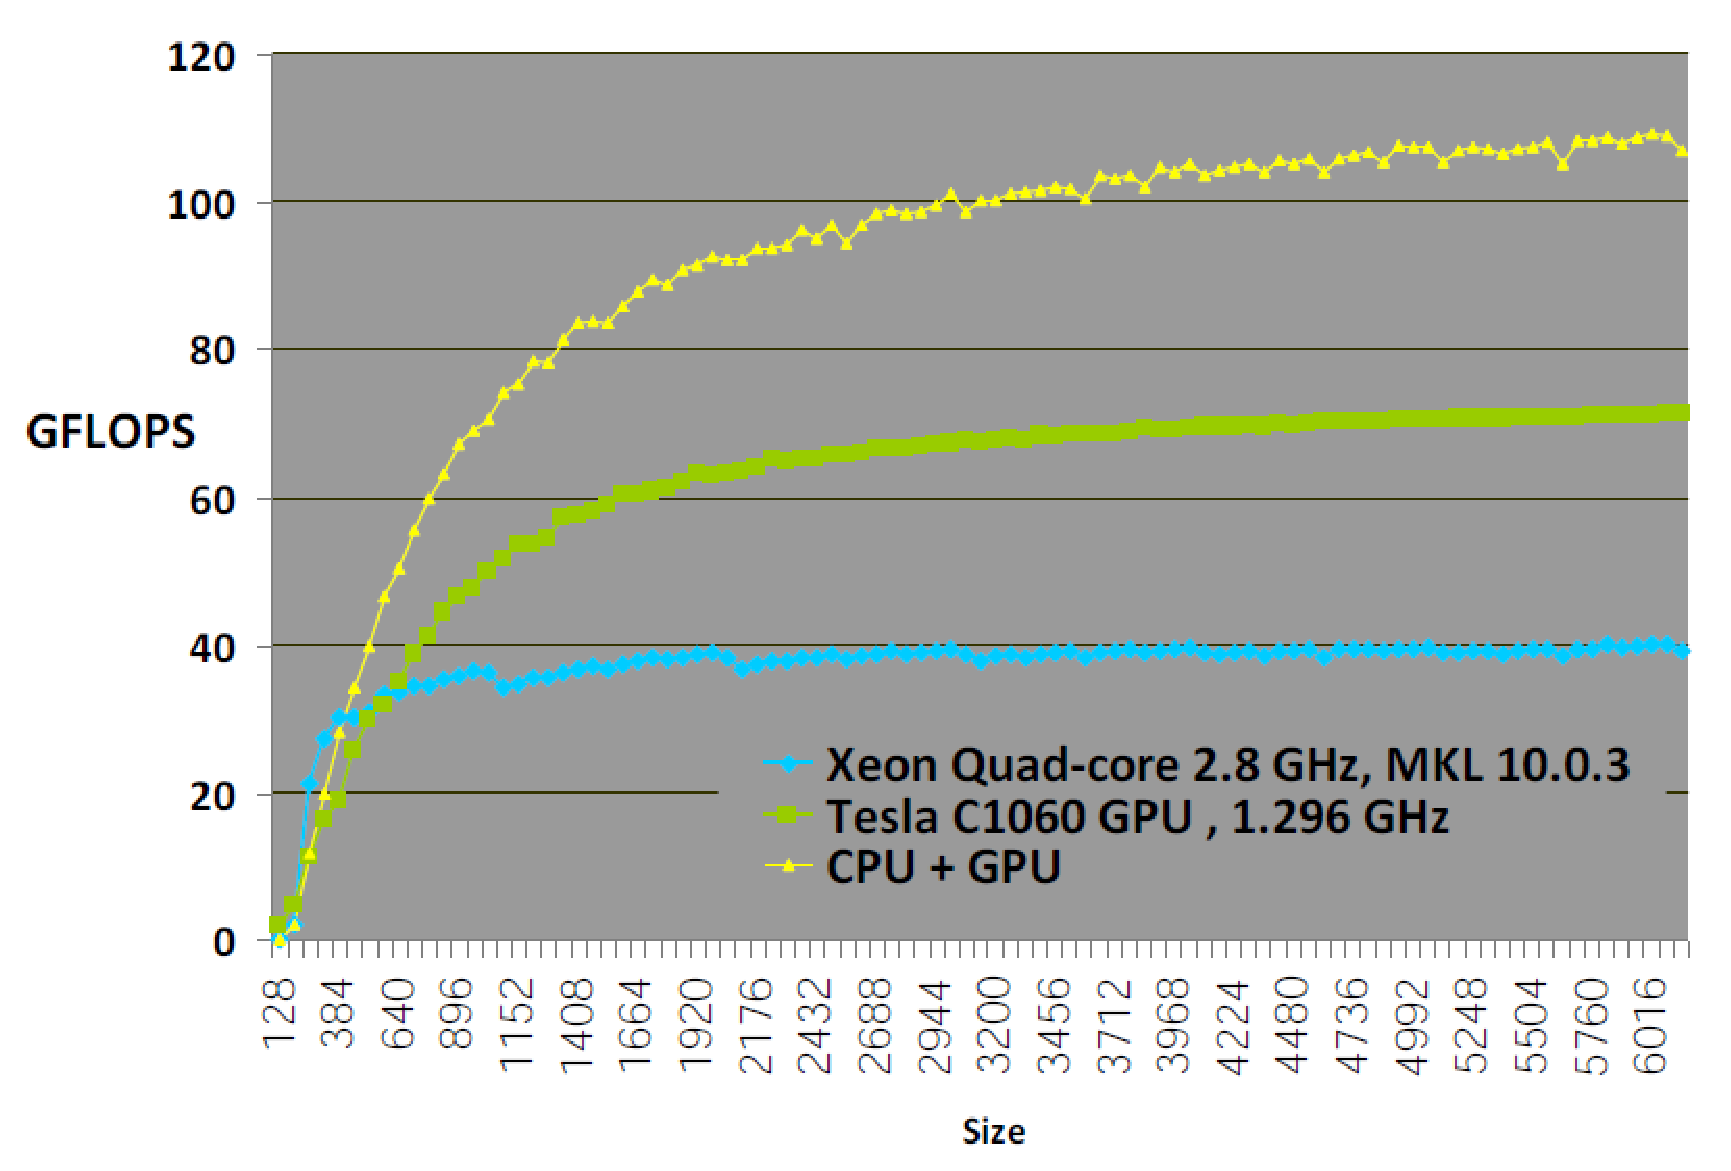
\includegraphics[height=5cm,
    angle=0]{./images/dgemm.eps}}
\caption{DGEMM}
\label{fig:dgemm_cublas}
\end{figure}
References:
\begin{itemize}
\item \url{http://www.gsic.titech.ac.jp/~ccwww/tebiki/tesla_e/tesla5_e.html}
\end{itemize}


%%% Local Variables: 
%%% mode: latex
%%% TeX-master: "gpucomputing"
%%% End: 
